\documentclass[12pt, a4paper]{article}

\usepackage[utf8]{inputenc}

% Limit the page margin to only 1 inch.
\usepackage[margin=1in]{geometry}

%Imports biblatex package
\usepackage[
backend=biber,
style=alphabetic
]{biblatex}
%\addbibresource{../../mth342.bib}

% Enables the `align' environment.
\usepackage{amsmath}

% Provides useful environments, such as:
% - \begin{proof} ...\end{proof}
\usepackage{amsthm}
\newtheorem*{proposition}{Proposition}
\theoremstyle{definition}
\newtheorem*{definition}{Definition}

% Enables using \mathbb{}, for example \mathbb{N} for the set of natural numbers.
\usepackage{amssymb}

% Allows using letters in enumerate list environment. Use, for example:
%\begin{enumerate}[label=(\alph*)]
% ...
%\end{enumerate}
\usepackage[inline]{enumitem}

% Enable importing external graphic files and provides useful commands, like \graphicspath{}
\usepackage{graphicx}
% Images are located in a directory called "images" in the current directory.
\graphicspath{{./images/}}

% Make links look better by default.
% See: https://tex.stackexchange.com/questions/823/remove-ugly-borders-around-clickable-cross-references-and-hyperlinks
\usepackage[hidelinks]{hyperref}
\usepackage{xcolor}
\hypersetup{
	colorlinks,
	linkcolor={red!50!black},
	citecolor={blue!50!black},
	urlcolor={blue!80!black}
}

% Code Listings. Source:
% https://stackoverflow.com/questions/3175105/inserting-code-in-this-latex-document-with-indentation
\usepackage{listings}
\usepackage{color}

\definecolor{dkgreen}{rgb}{0,0.6,0}
\definecolor{gray}{rgb}{0.5,0.5,0.5}
\definecolor{mauve}{rgb}{0.58,0,0.82}

\lstset{frame=tb,
	language=Java,
	aboveskip=3mm,
	belowskip=3mm,
	showstringspaces=false,
	columns=flexible,
	basicstyle={\small\ttfamily},
	numbers=none,
	numberstyle=\tiny\color{gray},
	keywordstyle=\color{blue},
	commentstyle=\color{dkgreen},
	stringstyle=\color{mauve},
	breaklines=true,
	breakatwhitespace=true,
	tabsize=3
}

\newcommand{\prob}{\text{P}}
%\newcommand{\complement}{\mathsf{c}}
\title{Lecture 6: MATH 342W: Introduction to Data Science and Machine Learning}
\author{Sergio E. Garcia Tapia\thanks{Based on lectures of Dr. Adam Kapelner at Queens College.
See also the \href{https://github.com/kapelner/QC_MATH_342W_Spring_2025}{course GitHub page}.}}
\date{February 13, 2025 (last updated \today)}

\begin{document}
	\maketitle
	\section*{Recap of Classification}
	Throughout our study, we have focused on the problem of binary classification, where there
	are two possible responses. That is, the response space is $\mathcal{Y}=\{0, 1\}$,
	and this is the context in which the \emph{Perceptron Learning Algorithm} (PLA) and
	the \emph{Support Vector Machine} (SVM) operate. A more general version of this problem
	allows for $L$ different classifications, so that $\mathcal{Y}=\{c_1,\ldots,c_L\}$,
	for some $L\in\mathbb{N}$,
	a problem known as \textbf{multinomial classification}. Due to lack of time, we will
	not be exploring this.
	\section*{$K$ Nearest Neighbors}
	Given a data set $\mathbb{D}$, recall that our motivation for obtaining 
	$g=\mathcal{A}(\mathbb{D},\mathcal{H})$ is to make predictions. That is,
	if $\mathcal{X}$ is our feature space, and we see an input $\mathbf{x}_*\in \mathcal{X}$
	that does not belong to $\mathbb{D}$, then we wish to predict the response as $g(\mathbf{x}_*)$.
	
	One way to predict the response for $\mathbf{x}_*$ is to find the \emph{closest} input
	$\mathbf{x}_k$ in $\mathbb{D}$ and to assign the response corresponding to $\mathbf{x}_k$
	as the prediction using the input $\mathbf{x}^*$. This is called the \textbf{nearest neighbor model}.
	That is, we let $g(\mathbf{x}_*) = y_k$. The meaning of \emph{closest} then becomes a
	hyperparameter, which is a \emph{distance function}:
	\begin{align*}
		d&:\mathcal{X}\times \mathcal{X}\to[0, \infty)\\
		d(\mathbf{u}, \mathbf{v}) &= \begin{cases}
			0 & \text{if } \mathbf{u} = \mathbf{v}\\
			\text{positive.} & \text{otherwise.}
		\end{cases}
	\end{align*}
	If $\mathcal{X}$ is a subset of $\mathbb{R}^p$, then a reasonable default is
	to let $d=\|\cdot \|_2$, the vector $2$-norm:
	\begin{align*}
		d(\mathbf{u}, \mathbf{v})=\|\mathbf{u} - \mathbf{v}\|_2
		=\sqrt{\sum_{j=1}^{p}(u_{j} - v_{j})^2}
	\end{align*}
	The main difficulty with this is that it is sensitive to the scale of the units
	of the inputs. For example, we get vastly different values when using nanometers vs. kilometers.
	This problem is typically addressed by normalizing to interval data, writing
	$x'=\frac{x-\bar{x}}{s}$. This adds a pre-processing step on our data set $\mathbb{D}$.
	
	Another issue is this: what if one of our sample points behaves strangely? For example, suppose
	that our data set contains information about credit history for people and whether they
	defaulted on a loan they took out. Though unlikely, one of our pairs on $(\mathbf{x}_i, y_i)$
	in $\mathbb{D}$ might correspond to a person whose observation $\mathbf{x}_i$ describes them as having
	a perfect credit history, but whose response $y_i$ was to default on their loan. What happens
	when a person $\mathbf{x}_*$ comes in with a perfect credit score, or more specifically,
	with features very similar to $\mathbf{x}_i$?  The approach we've described
	would determine that $\mathbf{x}_i$ is the closest point to $\mathbf{x}_*$, and would assign $g(\mathbf{x}_*)=y_i$. This is problematic, for example, if our data set contains many
	other points similar to $\mathbf{x}_i$ that had a different response, and perhaps one of those
	responses would have been more appropriate for $g(\mathbf{x}_*)$. To address this difficulty,
	we take not the closest $\mathbf{x}_i$, but the closest $k$ points $\mathbf{u}_1,\ldots,\mathbf{u}_k$
	(this is some permutation of the $\mathbf{x}$'s in $\mathbb{D}$), and take the mode:
	\begin{align*}
		g(\mathbf{x}_*)=\text{Mode}[g(\mathbf{u}_1),\ldots,g(\mathbf{u}_k)]
	\end{align*}
	This approach is called the \textbf{$k$-nearest neighbors} ($KNN$) model.
	This concludes (for now) our discussion of classification modeling.
	\section*{Regression Modeling}
	Suppose the response space is an interval or it's a ``numeric" response, meaning
	$\mathcal{Y}\subseteq \mathbb{R}$. Models with such a response space are called
	\textbf{``regression" models} (for historical reasons only). If $\mathcal{X}=\mathbb{R}$,
	then $\mathbb{D}$ is a set of points in the plane, which can be depicted with a
	\emph{scatterplot} (see Figure~\ref{fig:scatter-plot}).
	\begin{figure}
		\centering
		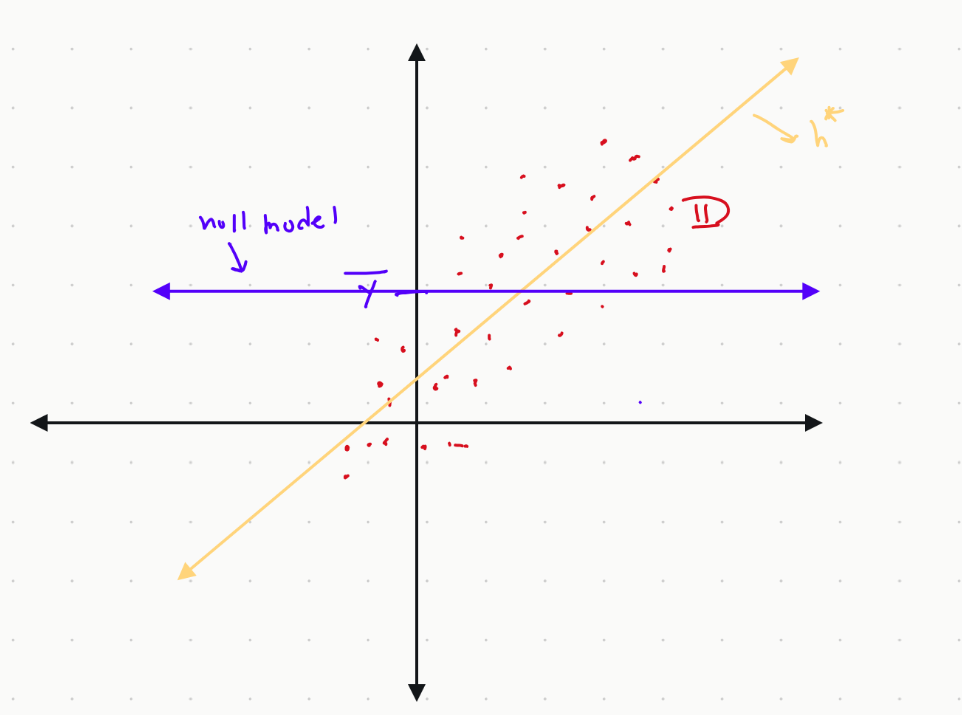
\includegraphics[width=0.6\textwidth]{scatter-plot-null-model}
		\caption{A scatterplot depicting a data set $\mathbb{D}$, the null model $g_0$,
		and $h^*$.}
		\label{fig:scatter-plot}
	\end{figure}
	
	If we do not know or see any features, the \emph{null model} in this context is
	the \emph{average}:
	\begin{align}
		g_0 = \bar{y}\label{eqn:null-model}
	\end{align}
	Recall the null model is meant to serve as a reference for performance. How can
	we beat it? A simple starting point is to let the set of candidate functions
	be the set of hyperplanes:
	\begin{align*}
		\mathcal{H} = \{\mathbf{w}\cdot\mathbf{x}=0: \mathbf{w}\in\mathbb{R}^{p+1},
		\mathbf{x}\in \{1\}\times \mathbb{R}^p\},
	\end{align*}
	where $\mathbf{x}$ has been extended to length $p+1$ by pre-pending  a 1
	entry.
	If the data set $\mathbb{D}$ does not suggest a linear pattern, we may see a high
	amount of misspecification error. Nevertheless, we will study this approach.
	The best candidate function $h^*$ is given by
	\begin{align*}
		h^*(\mathbf{x}) &= \mathbf{\beta}\cdot\mathbf{x}+\mathcal{E}\\
		&=\beta_0 + \beta_1x_1+\cdots+\beta_px_p+\mathcal{E}
	\end{align*}
	The vector $\mathbf{\beta}\in\mathbb{R}^{p+1}$ consists of the optimal weights that define a hyperplane
	that performs best with respect to the data set $\mathbb{D}$. The quantity $\mathcal{E}$
	is the error or noise. However, our algorithm will produce $g$, not $h^*$. In binary
	classification, we quantified the error as misclassification error. Here, we have
	a few choices:
	\begin{align*}
		SSE &:=  \sum_{i=1}^{n}e_i^2=\sum_{i=1}^{n}(y_i-\hat{y}_i)^2\quad \text{(Sum of Squared Errors)}\\
		SAE &:=  \sum_{i=1}^{n}|e_i|=\sum_{i=1}^{n}|y_i-\hat{y}_i|\quad \text{(Sum of Absolute Errors)}
	\end{align*}
	The $SSE$ is the default for practical reasons, as we will see. An algorithm
	that attempts to find the optimal $\mathbf{w}\in\mathbb{R}^{p+1}$, call it $\mathbf{b}$,
	that defines a hyperplane will attempt to minimize the $SSE$:
	\begin{align*}
		\mathcal{A}:\mathbf{b}=\underset{\substack{\mathbf{w}\in\mathbb{R}^{p+1}}}{\text{argmin}}
		\{SSE(\mathbf{\mathbf{w}})\}
	\end{align*}
	It looks difficult, but this is why we chose $SSE$; this has an analytical solution.
	We will focus on the case where $p=1$, and we will derive the general case in the future.
	\subsection*{Ordinary Least Squares Model (OLS)}
	If $p=1$, then $\mathbf{b}\in\mathbb{R}^2$, and
	\begin{align*}
		\hat{y}=g(x) = \mathbf{b}\cdot \mathbf{x}
		=\mathbf{b}^\top \mathbf{x}
		=\begin{bmatrix}
			b_0 & b_1
		\end{bmatrix}
		\begin{bmatrix}
			1 \\
			x
		\end{bmatrix}
		=b_0 + b_1x
	\end{align*}
	where $b_0$ is the $y$-intercept and $b_1$ is the slope. The objective function that we
	are trying to minimize is
	\begin{align*}
		SSE = \sum_{i=1}^{n}(y_i - \hat{y}_i)^2=\sum_{i=1}^{n}(y_i-w_0-w_1x_i)^2
	\end{align*}
	This is a function of two variables $w_0$ and $w_1$, whose optimal choice
	will be $w_0=b_0$ and $w_1=b_1$ (recall that we know $x_i$ and $y_i$,
	since they make up $\mathbb{D}$). Since $w_0$ and $w_1$ are unknowns, $SSE$
	is a function of $w_0$ and $w_1$. To minimize the $SSE$, we take the partial derivative with
	respect to each independent variable and set it to zero:
	\begin{align*}
		\frac{\partial}{\partial w_0}[SSE]&=\frac{\partial}{\partial w_0}
		\sum_{i=1}^{n}(y_i-w_0-w_1x_i)^2\\
		&=\sum_{i=1}^{n}\frac{\partial}{\partial w_0}(y_i-w_0-w_1x_i)^2
		\tag{by the linearity of the derivative}\\
		&=-2\sum_{i=1}^{n}(y_i-w_0-w_1x_i)
		\tag{by the Chain Rule}\\
		&=-2\left[\sum_{i=1}^{n}y_i - nw_0 - w_1\sum_{i=1}^{n}x_i\right]
	\end{align*}
	First we'll simplify notation by using the average of the $x$'s and $y$'s:
	\begin{align*}
		\bar{x}=\frac{\sum_{i=1}^{n}x_i}{n},\quad \bar{y}=\frac{\sum_{i=1}^{n}y_i}{n}
	\end{align*}
	Now  using this, we set the partial derivative to zero to find an extremum.
	We will denote $b_0$ and $b_1$ as the values of the parameters $w_0$ and $w_1$
	that allows the $SSE$ to achieve its extremum value:
	\begin{align}
		0 &= \frac{\partial}{\partial w_0}[SSE_0]\nonumber\\
		0&=-2\left[\sum_{i=1}^{n}y_i - nb_0 - b_1\sum_{i=1}^{n}x_i\right]\nonumber\\
		0&=-2(n\bar{y} - n b_0 - b_1n\bar{x})\nonumber\\
		b_0&=\bar{y}-b_1\bar{x}\label{eqn:b_0-parameter}
	\end{align}
	Since we have two variables $b_0$ and $b_1$, we need another equation, which we get by
	taking the partial derivative with respect to $w_1$. Once again, applying the Chain Rule and
	using the same notational simplification from earlier:
	\begin{align*}
		\frac{\partial}{\partial w_1}[SSE]
		&=\frac{\partial}{\partial w_1}\sum_{i=1}^{n}(y_i-w_0-w_1x_i)^2\\
		&=\sum_{i=1}^{n}-2x_i(y_i-w_0-w_1x_i)\\
		&=-2\left[\sum_{i=1}^{n}x_iy_i-nw_0\bar{x}-w_1\sum_{i=1}^{n}x_i^2\right]
	\end{align*}
	Setting the partial derivative to $0$ yields and using Equation~(\ref{eqn:b_0-parameter}):
	\begin{align}
		0 &= \frac{\partial}{\partial w_1}[SSE]\nonumber\\
		0&=-2\left[\sum_{i=1}^{n}x_iy_i-nb_0\bar{x}-b_1\sum_{i=1}^{n}x_i^2\right]\nonumber\\
		0&=\sum_{i=1}^{n}x_iy_i-nb_0\bar{x}-b_1\sum_{i=1}^{n}x_i^2\nonumber\\
		0&=\sum_{i=1}^{n}x_iy_i-n\bar{x}\bar{y}+nb_1\bar{x}^2-b_1\sum_{i=1}^{n}x_i^2\nonumber
		\tag{using Equation~\ref{eqn:b_0-parameter}}\\
		b_1\left(\sum_{i=1}^{n}x_i^2-n\bar{x}^2\right)&=\sum_{i=1}^{n}x_iy_i-n\bar{x}\bar{y}\nonumber\\
		b_1 &= \frac{\sum_{i=1}^{n}x_iy_i-n\bar{x}\bar{y}}{\sum_{i=1}^{n}x_i^2-n\bar{x}^2}\label{ref:b_1-parameter}
	\end{align}
	We can substitute this into Equation (\ref{eqn:b_0-parameter}) to get an expression
	for $b_0$. However, before that, we will change into a notation that is more compact,
	using language and notation from probability theory and statistics.
	Let
	\begin{align*}
		\rho := \text{Corr}[X, Y]:= \frac{\text{Cov}[X,Y]}{\text{SD}[X]\cdot \text{SD}[Y]}
		=\frac{\text{Cov}[X, Y]}{\sqrt{\text{Var}[X]\cdot \text{Var}[Y]}}
		:=\frac{\text{E}[(X-\mu_X)(Y-\mu_Y)]}{\sqrt{\text{Var}[X]\cdot \text{Var}[Y]}}
	\end{align*}
	where Corr stands for correlation, Cov stands for covariance, SD stands for standard deviation,
	Var stands for variance, and E stands for expectation. The estimate for $\rho$ is
	\begin{align*}
		r &:= \frac{S_{xy}}{S_{x}S_{y}},\\
		S_{xy} &:= \frac{1}{n-1}\sum_{i=1}^{n}(x_i-\bar{x})(y_i-\bar{y}),\\
		S_x^2 &:= \frac{1}{n-1}\sum_{i=1}^{n}(x_i-\bar{x})^2
	\end{align*}
	where $r$ is the \textbf{sample correlation}. Here, $S_{xy}$ is an estimate for the covariance,
	and $S_x^2$ is an estimate of variance. If we expand $S_{x,y}$, we get
	\begin{align*}
		S_{xy} &= \frac{\sum_{i=1}^{n}x_iy_i-\bar{y}\sum_{i=1}^{n}x_i-\bar{x}\sum_{i=1}^{n}y_i+\bar{x}\bar{y}}{n-1}\\
		&=\frac{\sum_{i=1}^{n}x_iy_i-\bar{y}\bar{x}-\bar{x}\bar{y}+\bar{x}\bar{y}}{n-1}\\
		&=\frac{\sum_{i=1}^{n}x_iy_i-n\bar{x}\bar{y}}{n-1}
	\end{align*}
	This looks like the numerator of $b_1$. Next, expanding $S_x^2$:
	\begin{align*}
		S_x^2 = \frac{\sum_{i=1}^{n}x_i^2 - n\bar{x}^2}{n-1}
	\end{align*}
	which looks like the denominator of $b_1$. Now:
	\begin{align*}
		b_1 &= \frac{\sum_{i=1}^{n}x_iy_i-n\bar{x}\bar{y}}{\sum_{i=1}^{n}x_i^2-n\bar{x}^2}\\
		&=\frac{(n-1)S_{xy}}{(n-1)S_x^2}
		=\frac{S_{xy}}{S_{x}^2}
		=\frac{rS_xS_y}{S_x^2}\\
		&=r\frac{S_y}{S_x}
	\end{align*}
	All of these formulas are valid and equivalent, though some are more pervasive than others. In short,
	we have the \textbf{simple/univariate least squares regression model}:
	\begin{align}
		b_0 &= \bar{y}-r\frac{S_y}{S_x}\bar{x}\\
		b_1 &= r\frac{S_y}{S_x}
	\end{align}
	The significance is that $g(x_*) = b_0 + b_1x_*$, which is an analytic solution
	(unlike our previous algorithms that required using an optimization from
	a package such as \texttt{optimx} in R). The parameters $b_0$ and $b_1$ define
	the $y$-intercept and slope, respectively, of the \textbf{least squares regression line}
	(think of a line of best fit, see Figure~\ref{fig:line-best-fit}.)
	\begin{figure}
		\centering
		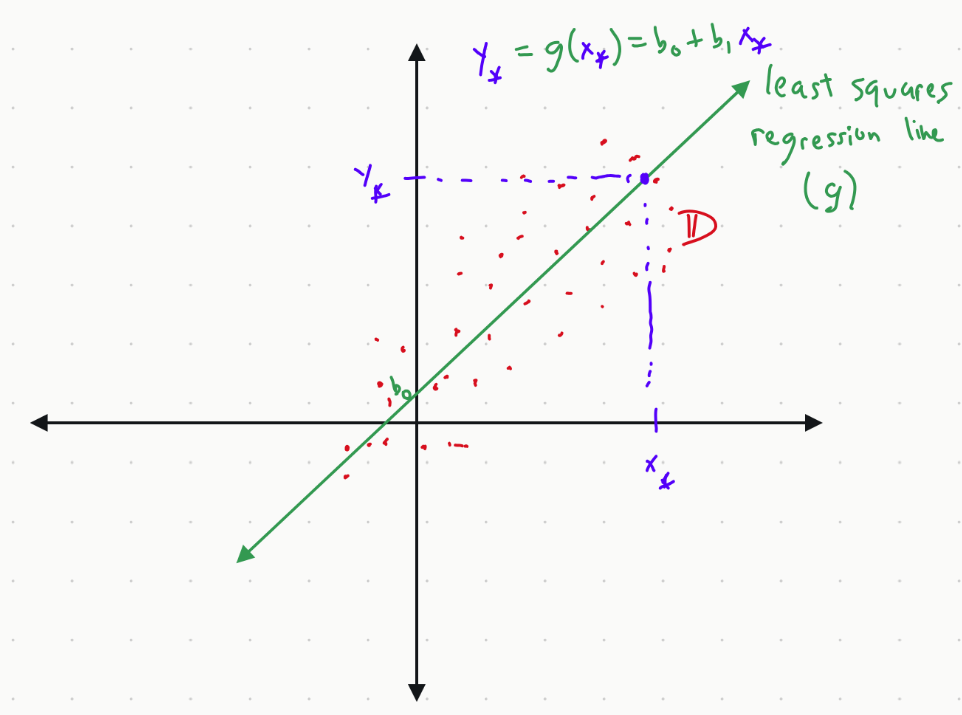
\includegraphics[width=0.6\textwidth]{least-squares-regression-line}
		\caption{The least squares regression line for a data set $\mathbb{D}$.}
		\label{fig:line-best-fit}
	\end{figure}
	\subsection*{Assessing the Quality of the Regression Model (Performance Metrics)}
	To see how well this model performs, we have the following options:
	\begin{enumerate}[label=(\arabic*)]
		\item \textbf{$SSE$}: The units of this quantity are response units squared.
		A disadvantage is that squared units are generally not intuitive (for example,
		what would squared dollars describe?). Also, $SSE$ is sensitive to $n$; as $n$
		increases, the $SSE$ also increases with $n$.
		\item \textbf{$MSE$}: One way to handle the scaling issue of $SSE$ is to use
		the \emph{mean squared error}:
		\begin{align*}
			MSE := \frac{1}{n-2}SSE
		\end{align*}
		Now this no longer scales with $n$, but it stills suffers from a lack of interpretability
		due to having squared units.
		\item \text{$RMSE$}: To get back to the response units, we can take the squared root:
		\begin{align*}
			RMSE :=\sqrt{MSE}
		\end{align*}
		This is the \emph{root mean squared error}. This addresses both the scaling issue
		and the units.
	\end{enumerate}
%	\printbibliography
\end{document}